
% Note for any github stalkers. I am currently in the process
% of learning LaTeX. I don't know what I'm doing yet. Sorry
% if my code absolutely sucks.


\documentclass{book}

\usepackage{fontspec} % used to import Calibri
\usepackage{anyfontsize} % used to adjust font size

% needed for inch and other length measurements
% to be recognized
\usepackage{calc}

% for colors and text effects as is hopefully obvious
\usepackage[dvipsnames]{xcolor}
\usepackage{soul}

% control over margins
\usepackage[margin=1in]{geometry}
\usepackage[strict]{changepage}

\usepackage{mathtools}
\usepackage{amsfonts}
\usepackage{amssymb} % originally imported to get the proof square

% Just am using this to get a dashed line in a table...
% Also you apparently want this to be inactive if you aren't
% using it because it slows compilation.
\usepackage{arydshln} \ADLinactivate 
\newenvironment{allowTableDashes}{\ADLactivate}{\ADLinactivate}

\usepackage{graphicx}
%\graphicspath{{./140A_images/}}

\usepackage{tikz}
   \usetikzlibrary{arrows.meta}
   \usetikzlibrary{graphs, graphs.standard}

\newfontfamily{\calibri}{Calibri}
\setlength{\parindent}{0pt}
\definecolor{RawerSienna}{HTML}{945D27}

\newcommand{\hOne}{%
   \color{Black}%
   \fontsize{14}{14}\selectfont%
}
\newcommand{\hTwo}{%
   \color{MidnightBlue}%
   \fontsize{13}{13}%
}
\newcommand{\hThree}{%
   \color{PineGreen}
   \fontsize{13}{13}
}
\newcommand{\hFour}{%
   \color{Cerulean}
   \fontsize{12}{12}
}
\newcommand{\myComment}{%
   \color{RawerSienna}%
   \fontsize{12}{12}%
}
\newcommand{\teachComment}{
   \color{Orange}%
   \fontsize{12}{12}%
}
\newcommand{\exOne}{%
   \color{Purple}%
   \fontsize{14}{14}\selectfont%
}
\newcommand{\exTwo}{%
   \color{RedViolet}%
   \fontsize{13}{13}\selectfont%
}
\newcommand{\exP}{%
   \color{VioletRed}%
   \fontsize{12}{12}\selectfont%
}

\newenvironment{myIndent}{%
   \begin{adjustwidth}{2.5em}{0em}%
}{%
   \end{adjustwidth}%
}

\newenvironment{myConstrict}{%
   \begin{adjustwidth}{2.5em}{2.5em}%
}{%
   \end{adjustwidth}%
}

\newcommand{\udefine}[1]{%
   \setulcolor{Red}%
   \setul{0.14em}{0.07em}%
   \ul{#1}%
}

\newcommand{\uuline}[2][.]{%
{\vphantom{a}\color{#1}%
\rlap{\rule[-0.18em]{\widthof{#2}}{0.06em}}%
\rlap{\rule[-0.32em]{\widthof{#2}}{0.06em}}}%
#2}

\newcounter{LectureNumber}
\newcommand*{\markLecture}[1]{%
   \stepcounter{LectureNumber}%
   {\huge \color{Black} \textbf{Lecture \theLectureNumber: #1} \newline}%
}

\newcommand{\pprime}{\prime\prime}

\newcounter{PropNumber}
\newcommand{\propCount}{%
   \stepcounter{PropNumber}%
   \thePropNumber%
}

\newcommand{\mySepOne}[1][.]{%
   {\noindent\color{#1}{\rule{6.5in}{1mm}}}\\%
}
\newcommand{\mySepTwo}[1][.]{%
   {\noindent\color{#1}{\rule{6.5in}{0.5mm}}}\\%
}

\newenvironment{myClosureOne}[2][.]{%
   \color{#1}%
   \begin{tabular}{|p{#2in}|} \hline \\%
}{%
   \\ \\ \hline \end{tabular}%
}

\newcommand{\retTwo}{\hfill\bigbreak}

\title{Math 158 Lecture Notes (Professor: Jacques Verstraete)}
\author{Isabelle Mills}


\begin{document}
   \maketitle
   \calibri

   \markLecture{1/9/2024}

   \hOne
   A \udefine{graph} is a pair $(V, E)$ where $V$ is a set of vertices
   and $E$ is a set of unordered pairs of elements of $V$ called edges.
   For $u, v \in V$, we say $u$ and $v$ are \udefine{adjacent} if 
   $\{u, v\} \in E$.

   
   \begin{center}
      \hTwo
      For example: $G = (\{1, 2, 3\}, \{\{1, 2\}, \{2, 3\}\})$
      
      % I'm so sorry I'm not using the packages I should be using
      % to draw these graphs. I haven't had time to learn them yet
      % and I want this section done at some point tonight before I go
      % to bed. 
      \hThree
      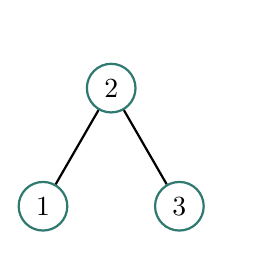
\begin{tikzpicture}
         \useasboundingbox (225:1.5) rectangle (45:2.5);

         \node (2) at (90:1) [circle, 
            draw=PineGreen!70!MidnightBlue, thick, fill=White] {2};
         \node (1) at (210:1) [circle, 
            draw=PineGreen!70!MidnightBlue, thick, fill=White] {1};
         \node (3) at (330:1) [circle, 
            draw=PineGreen!70!MidnightBlue, thick, fill=White] {3};
         \draw [thick] (1) -- (2);
         \draw [thick] (2) -- (3);
      \end{tikzpicture}
   \end{center}

\hOne
A \udefine{directed graph} (a.k.a a \udefine{digraph}) is a pair $(V, E)$ 
where $V$ is a set of vertices and $E$ is a set of ordered pairs 
of elements of $V$.
\begin{center}
   \hTwo
   For example: $G = (\{1, 2, 3\}, \{(1, 2), (2, 3)\})$

   \hThree
   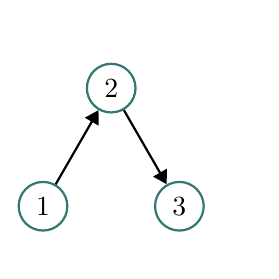
\begin{tikzpicture}
      \useasboundingbox (225:1.5) rectangle (45:2.5);

      \node (2) at (90:1) [circle, 
         draw=PineGreen!70!MidnightBlue, thick, fill=White] {2};
      \node (1) at (210:1) [circle, 
         draw=PineGreen!70!MidnightBlue, thick, fill=White] {1};
      \node (3) at (330:1) [circle, 
         draw=PineGreen!70!MidnightBlue, thick, fill=White] {3};
      \draw [thick, -Triangle] (1) -- (2);
      \draw [thick, -Triangle] (2) -- (3);
   \end{tikzpicture}
\end{center}

\hOne
A \udefine{multigraph} is a pair $(V, E)$ where $V$ is a set of vertices
and $E$ is a multiset of unordered pairs of elements of $V$.

\begin{center}
   \hTwo
   For example: $G = (\{1, 2, 3\}, \{\{1, 2\}, \{2, 3\}, \{2, 3\}\})$
   
   \hThree
   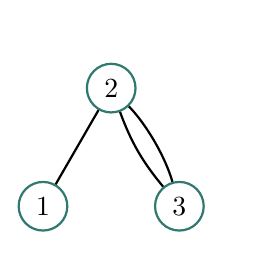
\begin{tikzpicture}
      \useasboundingbox (225:1.5) rectangle (45:2.5);

      \node (2) at (90:1) [circle, 
         draw=PineGreen!70!MidnightBlue, thick, fill=White] {2};
      \node (1) at (210:1) [circle, 
         draw=PineGreen!70!MidnightBlue, thick, fill=White] {1};
      \node (3) at (330:1) [circle, 
         draw=PineGreen!70!MidnightBlue, thick, fill=White] {3};
      \draw [thick] (1) -- (2);
      \draw [thick] (2) .. controls (50:.7) and (10:.7) .. (3);
      \draw [thick] (2) .. controls (50:.4) and (10:.4) .. (3);
   \end{tikzpicture}
\end{center}

\hOne
A \udefine{pseudograph} is like a graph and multigraph except that the
pairs in $E$ are multisets. 
\begin{myIndent}\begin{myIndent}\begin{myIndent}
\begin{myIndent}\begin{myIndent}
   \teachComment
   Essentially, an element $\{a, a\}$ can belong to $E$ in a 
   pseudograph. This type of edge is called a \udefine{loop}.
\end{myIndent}\end{myIndent}\end{myIndent}
\end{myIndent}\end{myIndent}

\begin{center}
   \hTwo
   For example: $G = (\{1, 2, 3\}, \{\{1, 2\}, \{2, 3\}, \{3, 3\}\})$
   
   \hThree
   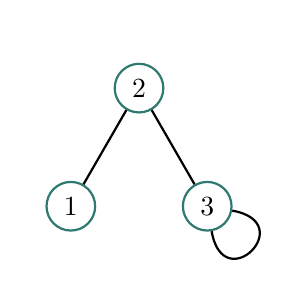
\begin{tikzpicture}
      \useasboundingbox (225:2) rectangle (45:2.5);

      \node (2) at (90:1) [circle, 
         draw=PineGreen!70!MidnightBlue, thick, fill=White] {2};
      \node (1) at (210:1) [circle, 
         draw=PineGreen!70!MidnightBlue, thick, fill=White] {1};
      \node (3) at (330:1) [circle, 
         draw=PineGreen!70!MidnightBlue, thick, fill=White] {3};
      \draw [thick] (1) -- (2);
      \draw [thick] (2) -- (3);
      \draw [thick] (3) to [out=350,in=280,looseness=6] (3);
   \end{tikzpicture}
\end{center}

\newpage
\hOne
If $G = (V, E)$ and $v \in V$, the \udefine{neighborhood} of $v$ is
$N_{G}(v)=\{w \in V \mid \{v, w\} \in E\}$. \bigbreak

The \udefine{degree} of $v$ is $d_{G}(v) = \lvert N_{G}(v) \rvert$.
Or in other words, $v$'s degree is equal to the number of edges 
connecting to $v$.

\mySepTwo[MidnightBlue]
\hTwo
\begin{myIndent}
   The \udefine{Handshaking lemma} states that for any graph $(V, E)$:
      {\fontsize{16}{15}\selectfont
      \[ \sum_{v \in V} d_{G}(v) = 2 \lvert E \rvert \]}
   
   \hThree
   \begin{myIndent}
      The reason for this is that each edge increments the degrees of
      exactly two vertices. So the above sum counts every edge twice.
      \hfill \bigbreak
   \end{myIndent}

   \hTwo
   \uuline{Lemma}: Every graph has an even number of vertices with odd
   degrees.

   \hThree
   \begin{myIndent}
      Proof: We can split the vertices of any graph into two categories:
      those with odd degrees, and those with even degrees.
      \hfill \bigbreak
      Now recall that an even number plus an even number always equals
      an even number, as does an odd number plus an odd number. However,
      an odd number plus an even numbers equals an odd number. Based on
      this fact, we can guarentee that the sum of even degrees in any
      graph is even. And since the sum of even degrees plus the sum of 
      odd\\ degrees must be even as it equals $2 \lvert E \rvert$ by
      the Handshaking lemma, we thus know that the sum of odd degrees 
      must be even. Hence, it must be the case that there are an even 
      number of vertices with odd degree because otherwise the sum of 
      their degrees won't be even.
      \hfill \bigbreak
   \end{myIndent}

   \hTwo
   A graph is called \udefine{$r$-regular} if all of its vertices have
   degree $r$.
   \hThree
   \begin{myIndent}
      Note that the number of edges in any $n$-vertex $r$-regular graph is
      $ \displaystyle{\frac{rn}{2}}$.
      \hfill \bigbreak
   \end{myIndent}
   
   \hTwo
   An $r$-dimensional \udefine{cube graph}, denoted as $\mathrm{Q}_{r}$,
   is a graph such that $V(\mathrm{Q}_{r})$, the set of vertices in 
   $\mathrm{Q}_{r}$, is equal to the set of binary strings of 
   length $r$; and $E(\mathrm{Q}_{r})$, the set of edges in 
   $\mathrm{Q}_{r}$, is equal to the set of pairs of binary strings
   which differ in only one position.

   \begin{center}
      \begin{tabular}{ c c }
         \hThree \fontsize{10}{10}\selectfont
         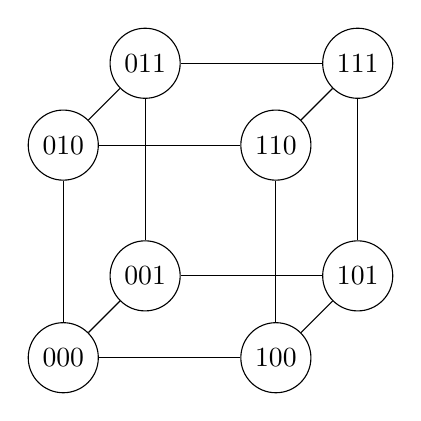
\begin{tikzpicture}[scale=0.9]
            \tikzstyle{myCir}=[circle,draw];
            \node[myCir] (000) at (0,0,0) {000};
            \node[myCir] (100) at (3,0,0) {100} edge (000);
            \node[myCir] (010) at (0,3,0) {010} edge (000);
            \node[myCir] (110) at (3,3,0) {110} edge (010) 
                                             edge (100);
            \node[myCir] (001) at (0,0,-3) {001} edge (000);
            \node[myCir] (101) at (3,0,-3) {101} edge (100) 
                                             edge (001);
            \node[myCir] (011) at (0,3,-3) {011} edge (010)   
                                             edge (001);
            \node[myCir] (111) at (3,3,-3) {111} edge (110) 
                                             edge (011) edge (101);
         \end{tikzpicture}
         & \hTwo
         ${\displaystyle \quad\quad\quad
         \begin{matrix}
            \lvert V(\mathrm{Q}_{r})\rvert = 2^{r} \\ \\
            \lvert E(\mathrm{Q}_{r})\rvert = \frac{2^{r}r}{2} = 
               2^{r-1}r \\ \\ \\ \\{\teachComment\text{
                  Note that } \mathrm{Q}_{r} \text{ is } r
                  \text{-regular.}}
         \end{matrix}}$
      \end{tabular}
   \end{center}
\end{myIndent}

\hOne
If $G=(V, E)$, then $H=(W, F)$ is a \udefine{subgraph} of $G$
if $W\subseteq V$ and $F\subseteq E$. \retTwo

If $W=V$, then $H$ is a \udefine{spanning subgraph} of $G$ (meaning 
that $H$ has the same vertices as $G$ but is lacking some of $G$'s 
edges) \retTwo

We define subtracting a set of vertices from a graph as follows:
\begin{myIndent} \hTwo
   For $G = (V, E)$ and $X \subset V$, we define...
      \begin{myIndent}\begin{myIndent}
         ${\displaystyle G - X = (V \setminus X, \{\{u, v\}\in E 
         \mid \{u, v\}\cap X = \emptyset\}) }$
      \end{myIndent}\end{myIndent}
\end{myIndent}
\retTwo

\hOne % I might not actually need this command here...
We define subtracting a set of edges from a graph as follows:
\begin{myIndent} \hTwo
   For $G = (V, E)$ and $L \subset E$, we define...
      \begin{myIndent}\begin{myIndent}\begin{myIndent}\begin{myIndent}
         ${\displaystyle G - L = (V, E \setminus L) }$
      \end{myIndent}\end{myIndent}\end{myIndent}\end{myIndent}
\end{myIndent} \retTwo

\hOne \markLecture{1/11/2024} \retTwo

We shall notate that $H$ is a subgraph of $G$ by 
writing $H \subseteq G$. \retTwo

An \udefine{induced subgraph} of $G = (V, E)$ is a subgraph 
$G\left[ X \right] = G - (V \setminus X)$ where $X \subseteq V$.
Alternatively, this is called the subgraph induced by $X$.
\retTwo

% Augh there is a bug with the uuline command I made!!!!
Given $G = (V, E)$ and $F \subseteq E$, the 
\udefine{subgraph spanned by $F$} is the subgraph whose edge set is $F$ 
and whose vertex set is ${\displaystyle
\bigcup_{e \in F}e}$. \retTwo

\mySepTwo \hOne
\begin{myIndent}\begin{myIndent}\begin{myIndent}\begin{myIndent}
   Here are some basic classes of graphs: \retTwo
\end{myIndent}\end{myIndent}\end{myIndent}\end{myIndent}

   \begin{itemize}
   \item \udefine{Complete graphs / cliques}, denoted $K_n$, are graphs 
      where every possible edge is present between $n$ vertices.\hTwo

      \begin{center}
      \begin{allowTableDashes}\begin{tabular}
                           { c;{10pt/3pt}c;{10pt/3pt}c;{10pt/3pt}c c c }

         \begin{tikzpicture}[scale=0.5, inner sep=3pt]
            \useasboundingbox (-1.5,-3.5) rectangle (1.5,3);

            \tikzstyle{myCir}=[circle,fill];
            \node[myCir] (1) at (0:0) {};
            \node (name) at (270:3) {$K_1$};
         \end{tikzpicture}

         &

         \begin{tikzpicture}[scale=0.5, inner sep=3pt]
            \useasboundingbox (-3,-3.5) rectangle (3,3);

            \tikzstyle{myCir}=[circle,fill];
            \node[myCir] (1) at (0:2) {};
            \node[myCir] (2) at (180:2) {} edge (1);
            \node (name) at (270:3) {$K_2$};
         \end{tikzpicture}

         &

         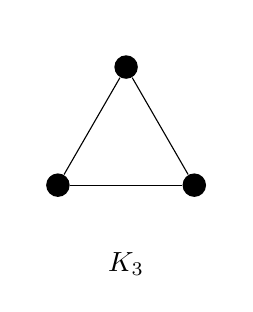
\begin{tikzpicture}[scale=0.5, inner sep=3pt]
            \useasboundingbox (-2.5,-3.5) rectangle (2.5,3);

            \tikzstyle{myCir}=[circle,fill];
            \node[myCir] (1) at (330:2) {};
            \node[myCir] (2) at (210:2) {} edge (1);
            \node[myCir] (3) at (90:2) {} edge (1) edge (2);
            \node (name) at (270:3) {$K_3$};
         \end{tikzpicture}

         &

         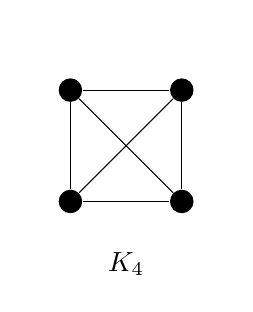
\begin{tikzpicture}[scale=0.5, inner sep=3pt]
            \useasboundingbox (-2.5,-3.5) rectangle (2.5,3);

            \tikzstyle{myCir}=[circle,fill];
            \node[myCir] (1) at (45:2) {};
            \node[myCir] (2) at (135:2) {} edge (1);
            \node[myCir] (3) at (225:2) {} edge (1) edge (2);
            \node[myCir] (4) at (315:2) {} edge (1) edge (2) edge (3);

            \node (name) at (270:3) {$K_4$};
         \end{tikzpicture}
      \end{tabular} \end{allowTableDashes}
      \end{center}

      
      \begin{myIndent}\begin{myIndent}\begin{myIndent}\begin{myIndent}
         \teachComment \begin{tabular}{ p{2.75in} c }
            
            Note we can also draw $K_4$ such that there are no edge
            interceptions as follows: &
         {\raisebox{-2.5em}{\tikz[scale=0.5, inner sep=3pt]{
            \tikzstyle{myCir}=[circle,fill];
            \node[myCir] (1) at (330:2) {};
            \node[myCir] (2) at (210:2) {} edge (1);
            \node[myCir] (3) at (90:2) {} edge (1) edge (2);
            \node[myCir] (4) at (0:0) {} edge (1) edge (2) edge (3);
         }}}
         \end{tabular}
      \end{myIndent}\end{myIndent}\end{myIndent}
      
      \hTwo
      $\lvert V(K_n) \rvert = n$ \\
      $\lvert E(K_n) \rvert = \begin{pmatrix} n
         \vphantom{\frac{1}{1}} \\ 2\vphantom{\frac{
         \frac{1}{1}}{1}} \end{pmatrix} = \dfrac{n(n - 1)}{2}$ \retTwo
      \end{myIndent}
      \newpage

      \hOne
      \item A graph $G = (V, E)$ is bipartite if there exists a
         partition $(A, B)$ of $V$ such that every edge in $E$
         has one end in $A$ and one end in $B$. \retTwo
         {\hTwo \begin{tabular}{p{2in} p{0.5in} p{3in}}
            \raisebox{-6em}{
               \tikz[scale=0.6, inner sep=3pt]{
                  \tikzstyle{myCir}=[circle, fill];

                  \draw[color=VioletRed, thick] 
                              (0, -1) arc (270:630:0.6 and 3);
                  \node (t) at (-1.25, 2) {{\color{VioletRed}\Huge A}};
                  
                  \draw[color=VioletRed, thick] 
                              (4, 0) arc (270:630:0.6 and 2);
                  \node (t) at (5.25, 2) {{\color{VioletRed}\Huge B}};
                  
                  \node[myCir] (t1) at (4,3) {};
                  \node[myCir] (t2) at (4,1) {};
                  \node[myCir] (s1) at (0,4) {} edge (t1) edge (t2);
                  \node[myCir] (s2) at (0,2) {} edge (t1);
                  \node[myCir] (s3) at (0,0) {} edge (t2); 
               }
            }
            &
            & 
            {The partition $(A, B)$ is called the \newline
            \udefine{bipartition} of $G$. Then $A$ and $B$ are called 
            the \udefine{parts} of $G$.}
         \end{tabular}} \retTwo

      \item A \udefine{Complete bipartite graphs} $K_{s,t}$, is the 
         bipartite graph with parts $A$ and $B$ where 
         $\lvert A \rvert = s$, $\lvert B \rvert = t$, and all 
         possible edges between $A$ and $B$ exist.

         \begin{myIndent}\begin{myIndent} \hTwo
            For example, $K_{3,2}$: \hspace{2em} \raisebox{-2.3em}{
               \tikz[scale=0.5, inner sep=3pt]{
                  \tikzstyle{myCir}=[circle, fill];
                  \node[myCir] (t1) at (4,3) {};
                  \node[myCir] (t2) at (4,1) {};
                  \node[myCir] (s1) at (0,4) {} edge (t1) edge (t2);
                  \node[myCir] (s2) at (0,2) {} edge (t1) edge (t2);
                  \node[myCir] (s3) at (0,0) {} edge (t1) edge (t2); 
               }
            }
         \end{myIndent}\end{myIndent} \retTwo
   
      \item A \udefine{path} $P_k$ of length $k$ has a vertex set
         $V = \{v_1, v_2, \ldots, v_k, v_{k+1}\}$ and an edge set
         $E = \{\{v_1, v_2\}, \{v_2, v_3\}, \ldots, 
         \{v_{k-1}, v_k\}, \{v_k, v_{k+1}\}\}$.
      
         {\center \hTwo
            Note that $\lvert V(P_k) \rvert = k+1$ and $\lvert E(P_k) 
            \rvert = k$. \\ Therefore, below would be $P_3$...
         
            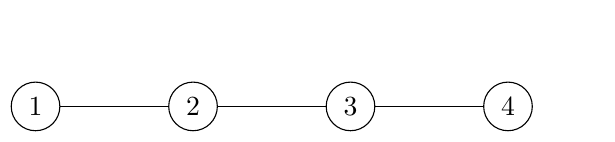
\begin{tikzpicture}
               \tikzstyle{myCir}=[circle, draw]

               \useasboundingbox (-0.1,-0.1) rectangle (7,1);

               \node[myCir] (4) at (6,0) {4};
               \node[myCir] (3) at (4,0) {3} edge (4);
               \node[myCir] (2) at (2,0) {2} edge (3);
               \node[myCir] (1) at (0,0) {1} edge (2);
            \end{tikzpicture} \retTwo
         
         \par }
      
      \item A \udefine{cycle} $C_k$ of length $k$ has a vertex set 
         $V = \{v_1, v_2, \ldots, v_k\}$ and an edge set $E = 
         \{\{v_1, v_2\}, \{v_2, v_3\}, \ldots, \{v_{k-1}, v_k\},
            \{v_k, v_1\}\}$.
         
         {\center \hTwo
            Note that $\lvert V(C_k) \rvert = k$ and $\lvert E(C_k) 
            \rvert = k$. \\ Therefore, below would be $C_4$...

            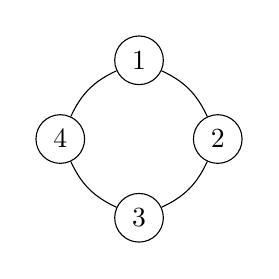
\begin{tikzpicture}[scale=0.5]
               \tikzstyle{myCir}=[circle, draw]

               \useasboundingbox (225:4) rectangle (45:4);

               \node[myCir] (2) at (0:2) {2};
               \node[myCir] (1) at (90:2) {1} edge [bend left=20] (2);
               \node[myCir] (4) at (180:2) {4} edge [bend left=20] (1);
               \node[myCir] (3) at (270:2) {3} edge [bend left=20] 
                        (4) edge [bend right=20] (2);
            \end{tikzpicture} \retTwo
         \par}

\end{itemize}
\newpage
Here is some terminology before the next lemma. For the graph
$G = (V, E)$\ldots
   
   \begin{itemize}
      \item $\delta(G) = \min\{d_G(v) \mid v \in V\}$ is the 
      \udefine{minimum degree} of $G$.
      \item $\Delta(G) = \max\{d_G(v) \mid v \in V\}$ is the 
      \udefine{maximum degree} of $G$.
      \item The \udefine{degree sequence} of $G$ is the 
      sequence of degrees of vertices $G$ in \\non-increasing order.
   \end{itemize}


\exOne
\begin{center}
\begin{myClosureOne}{5.5}
   \uuline{Lemma (part 1)}: If $G = (V, E)$ is a graph of minimum degree
   $k \geq 2$, then $G$ contains a cycle of length at least
   $k + 1$.

   {\exP \begin{myConstrict}
      Proof: Let $P$ be a longest possible path in $G$, say:
      \[V(P) = \{v_1, v_2, \ldots, v_r\}\]

      Then $N(v_r) \subseteq V(P)$. After all, if this were not 
      the case, we'd be able to extend the path to the vertex in 
      $N(v_r)$ but not in $V(P)$, thus contradicting the fact that
      $P$ is a longest path. \retTwo

      Let $v_i$ be the first neighbor of $v_r$ along the path from
      $v_1$ to $v_r$. Then $\{v_i, v_{i+1}, \ldots, v_r\}$ are the
      vertices of a cycle $C$. \retTwo

      Now note that because $N(v_r) \subseteq P$ and $v_i$ was
      the first element in the path $P$ to belong to $N(v_r)$, 
      we know that $C$ contains all the elements of $P$ that 
      $N(v_r)$ also has. So, $N(v_r) \subseteq C$. \retTwo

      But now note that $\lvert N(v_r) \rvert \geq \delta(G)=k$. Plus,
      $v_r$ itself is not in $N(v_r)$. Combining these facts together,
      we can say that the cycle $C$ has at least $k + 1$ vertices.
   \end{myConstrict}}

   \uuline{Lemma (part 2)}: The cycle length $k+1$ is the longest 
   we can guarentee based on the minimum degree of the graph being $k$.

   {\exP \begin{myConstrict}
      Proof: Take the graph $K_{k+1}$ which has a minimum degree $k$. 
      \newline
      Obviously, the longest cycle in $K_{k+1}$ is the cycle containing
      all $k+1$ elements of $K_{k+1}$. Thus, we have shown that there
      are graphs with minimum degree $k$ which don't have cycles of
      length greater than \newline $k + 1$.
   \end{myConstrict}} 
\end{myClosureOne}
\end{center}
\retTwo

\hOne
A \udefine{connected graph} is a graph in which any two vertices
are the ends of a path. \retTwo

The \udefine{components} of a graph are the \uuline{maximal connected
subgraphs}. For example: \retTwo
{\hTwo
   \begin{myIndent}\begin{myIndent}
      Let us define $G$ as: \hspace{2em}
      \raisebox{-2em}{\tikz[scale=0.4, inner sep=3pt]{
         \tikzstyle{myCir}=[circle, fill];
   
         \node[myCir] (t1) at (0, 1) {};
         \node[myCir] (t2) at (2, 1) {} edge (t1);
         \node[myCir] (t3) at (1, 3) {} edge (t1) edge (t2);
   
         \node[myCir] (y1) at (6, 2) {};
         \node[myCir] (y2) at (5, 4) {} edge (y1);
         \node[myCir] (y3) at (7, 4) {} edge (y1);
         \node[myCir] (y4) at (6, 0) {} edge (y1);
   
         \node[myCir] (p) at (10, 2) {};
   
         \draw[color=PineGreen, thick] 
                                 (-1.2, 2) arc (180:540:6 and 3);
      }} \retTwo

      As can be seen, $G$ has three components.
   \end{myIndent}\end{myIndent}
}
\newpage

A \udefine{tree} is a connected graph with no cycles
   (a.k.a it is acyclic). \hTwo
   \begin{myIndent}
      Some examples of small trees include: $K_1$, $K_2$, $K_{1,2}$, 
      $P_3$, and $K_{1,3}$.
   \end{myIndent}

   \begin{center}
      \begin{myClosureOne}{5.5}
         \uuline{Lemma}: Every tree with $n$ vertices has exactly
         $n - 1$ edges.
         \hThree
         \begin{myConstrict}
            Proof: We shall proceed by induction. \retTwo
            
            If $n = 1$, the tree is $K_1$, meaning that it has $0=n-1$
            edges. \retTwo

            Now assume the lemma is true for all trees with $n$
            vertices, and let $T$ be a tree with $n+1$ vertices. Then,
            we shall \newline remove a vertex $v$ of $T$ with degree $1$. 
            (Note that we know such a vertex must exist since 
            otherwise the \newline minimum degree of $T$ would be 
            at least $2$ and that would guarentee a cycle exists 
            of at least length 3. This
            of course contradicts the fact that $T$ is acyclic.)
            \retTwo 
            Then $T - \{v\}$ is a tree with $n$ vertices, 
            so by induction it has $n-1$ edges. And because
            $v$ has degree $1$, we know that $\lvert E(T) \rvert
            = 1 + \lvert E(T - \{v\}) \rvert = 1 + (n - 1) = n$.
         \end{myConstrict} \retTwo
         \hTwo

         \uuline{Lemma}: Any connected graph has a spanning tree.
         \hThree
         \begin{myConstrict}
            Proof: \retTwo

            Firstly consider the case that the graph $G$ has no cycle.
            Then, it is a tree by definition. \retTwo

            Now, consider if $G$ has a cycle $C$. Then for any edge \newline
            $e \in E(C)$, we have that $G - \{e\}$ is still connected.
            So, we can now go back to the top of the proof and ask:
            does $G -\{e\}$ have any cycles? We can repeatedly do this
            until the graph has no cycles since taking away edges
            does not remove any vertices.
            
         \end{myConstrict}
         \teachComment
         \begin{myIndent}\begin{myIndent}
            \begin{myConstrict}
            This actually acts as an algorithm for finding a spanning
            tree of any connected graph.
            \end{myConstrict}
         \end{myIndent}\end{myIndent}
      \end{myClosureOne}
   \end{center}\retTwo

\hOne

\begin{tabular}{ p{2in} p{1in} p{2.5in}}
   If $u$ and $v$ are two vertices in a connected graph, the
   \udefine{distance} from $u$ to $v$ is the length of a shortest
   path with ends at $u$ and $v$. & &
   \begin{centering} \hfill
      \raisebox{-6em}{\tikz[scale=0.9, inner sep=3pt, Black, very thick]{
            \tikzstyle{myCir}=[circle, fill];
            \tikzstyle{orng}=[color=Orange, line width=6pt, opacity=0.5];
      
            \node[myCir] (1) at (0, 0) {};
            \node[myCir] (2) at (2, 1) {} edge (1) edge[orng] (1);
            \node[myCir] (3) at (2, -1) {} edge (1) edge[orng] (1);
            \node[myCir] (4) at (3, 2) {} edge (2);
            \node[myCir, color=Red, label=above:{\color{red}$u$}] 
                  (5) at (4, .5) {} edge (2) edge[orng] (2);
            \node[myCir, color=Red, label=below:{\color{red}$v$}] 
                  (6) at (4, -.5) {} edge (3) edge[orng] (3);
            \node[myCir] (7) at (3, -2) {} edge (3);
            \node[myCir] (8) at (6, 1) {} edge (5);
            \node[myCir] (9) at (6, -1) {} edge (6);
         }}
   \end{centering}
\end{tabular}
\newpage

\hOne
Let $d_G(u, v)$ be the distance between $u$ and $v$.\retTwo

Distance is a \udefine{metric}, meaning:
\begin{myIndent}\begin{myIndent}\begin{enumerate}
   \item $d_G(u, v)=0 \Longleftrightarrow u=v$
   \item $d_G(u, v)=d_G(v, u)$
   \item $\forall w\in V, \hspace{0.5em}
      d_G(u, v) \leq d_G(u, w) + d_G(w, v)$
\end{enumerate}\end{myIndent}\end{myIndent} \retTwo

The \udefine{diameter} of a connected graph $G$ is the maximum distance
between any two vertices of $G$. Or in other words,
$\max\{d_G(u,v) \mid u,v\in  V(G)\}$. \retTwo

The \udefine{radius} of $G$ is equal to 
   $ \min\{\max\{d_g(u,v) \mid u\in V(G)\} \mid v\in V(G)\} $. What
   that means is that the radius of $G$ measures the smallest distance
   path one could limit themselves to drawing while still being able
   to have that path have one end at some fixed vertex and its other
   end at any arbitrary vertex in the graph.


\begin{myIndent}
   \hTwo \uuline{Examples}:
   \begin{enumerate}
      \item The radius of $K_n$  is $1$. The diameter of $K_n$ is $n$.
      \retTwo
      \item The diameter of $P_k$ is $k$. The radius, can be computed as
         follows:
         \begin{myIndent} \hFour
            The middle vertex of a path will have the fastest access
            to either end of the path. So, we shall measure the radius
            from the vertex: $v_{\lceil \frac{k+1}{2} \rceil}$. Then,
            we can see that $v_{k+1}$ is going to be a farthest element
            from $v_{\lceil \frac{k+1}{2} \rceil}$. So the radius
            of $P_k$ equals $k + \lceil \frac{k+1}{2} \rceil$.
            \retTwo

            Now you can consider what happens when $k$ is even and odd.
            But what's important is that it works out that the radius
            is $\lceil \frac{k}{2} \rceil$.
         \end{myIndent}
   \end{enumerate}
\end{myIndent} \retTwo
\hOne
We can use a \udefine{search tree} to more generally find
the radii and diameters of graphs. \retTwo

\begin{myIndent} \hTwo
   \uuline{Breadth-First-Search}
   \begin{myIndent}
      Here's how to find a spanning tree in a connected graph with a root
      vertex $v$ such that the tree "preserves" all distances
      from $v$.
      (This tree is called a \udefine{BFS tree}).
      \begin{myIndent} \hThree
         Let $G$ be a connected graph and let $(v_1, v_2, v_3,
         \ldots, v_n)$ be any \\ordering of the vertices of $G$.
         \retTwo
         Pick a vertex $v=v_1$ to be the root of the BFS-tree.
         \retTwo
         Now, at any stage in constructing this tree, we will have
         a vertex set $V(T) = \{v_1, v_2 \ldots, v_k\}$ (when we first
         start, $V(T)$ will only \\contain $v_0$. So don't worry about that).
         Now if $V(T)=V(G)$ we can stop. Otherwise though, we can say 
         that there is a smallest integer $i$ such that for $v_i \in V(T)$, 
         $\hspace{0.25em} N(v_i)\setminus V(T) \neq \emptyset$.
         Choose $v_{k+1}$ to be the smallest neighbor of $v_i$ 
         not in $T$ in the ordering of the vertices of $G$ and add 
         the edge $\{v_i, v_{k+1}\}$ to $T$. Then we repeat this paragraph.
         \retTwo
         Beware the ordering we are creating in our tree will often
         be different from the order of the graph you started with.
      \end{myIndent}
   \end{myIndent}
      \newpage
      \exOne

      
   \begin{center}\begin{myClosureOne}{5.5}
      \uuline{Worked Demonstration}: \retTwo
      \exTwo
      \begin{tabular}{ c c c }
         \begin{centering}
            \raisebox{-5em}{\tikz[scale=0.45,inner sep=4pt]{
               \tikzstyle{myCir}=[circle, draw];

               \node[myCir] (9) at (18:2) {9};
               \node[myCir] (7) at (90:2) {7};
               \node[myCir] (8) at (162:2) {8}
                  edge (9);
               \node[myCir] (3) at (234:2) {3}
                  edge (9) edge(7);
               \node[myCir] (10) at (306:2) {10}
                  edge (7) edge(8);
               \node[myCir] (5) at (18:5) {5}
                  edge (9);
               \node[myCir] (6) at (90:5) {6}
                  edge (7) edge (5);
               \node[myCir] (2) at (162:5) {2}
                  edge (6) edge (8);
               \node[myCir] (1) at (234:5) {1}
                  edge (2) edge (3);
               \node[myCir] (4) at (306:5) {4}
                  edge (1) edge (10) edge (5);
            }\par}
         \end{centering}
         &
         becomes
         &
         \begin{centering}
            \raisebox{-5em}{\tikz[scale=0.45,inner sep=4pt]{
               \tikzstyle{myCir}=[circle, draw];

               \node[myCir] (9) at (18:2) {9};
               \node[myCir] (7) at (90:2) {7};
               \node[myCir] (8) at (162:2) {8};
               \node[myCir] (3) at (234:2) {3}
                  edge (7) edge (9);
               \node[myCir] (10) at (306:2) {10};
               \node[myCir] (5) at (18:5) {5};
               \node[myCir] (6) at (90:5) {6};
               \node[myCir] (2) at (162:5) {2}
                  edge (6) edge (8);
               \node[myCir] (1) at (234:5) {1} 
                  edge (2) edge (3);
               \node[myCir] (4) at (306:5) {4}
                  edge (1) edge (5) edge (10);
            }\par}
         \end{centering}
      \end{tabular}
   \end{myClosureOne}\end{center} \retTwo

   \hTwo
   \begin{myIndent}
      \uuline{Properties of BFS}: \hfill \bigbreak

      \begin{itemize}
         \item If the root is $v$, then $d_T(v, w) = d_g(v, w)$
         \item The Tree has layers which are $N_i(v)=\{w\in V(G) \mid 
         d_G(v, w)=i\}$ and all edges in the tree and the graph are
         in some $N_i(v)$ or between $N_i(v)$ and $N_{i+1}(v)$.
         \item The diameter of $G$ equals the maximum number of
         layers of all BFS trees (not including the 0-layer).
         \item The radius of $G$ equals the minimum number of layers
         of all BFS trees (also not including the 0-layer).
      \end{itemize}
   \end{myIndent}

      
   
\end{myIndent}

\end{document}